\chapter{Sample Control Module} \label{sec:SampleControl}
The Sample Control module is the module responsible for generating the necessary inputs for a DAC that will generate the DUT input test signals and for controlling the ADCs that are sampling the resulting DUT voltage and current waveforms simultaneously. The module will take the samples from the ADCs and store them in external memory. The external memory can be accessed by the Main Processor module in order to retrieve and analyze the samples. The Sample Control module will recieve test parameters from the Main Processor and store them in internal registers, these internal registers are connected to the internal sample control logic and can be used to adjust the sampling parameters. The block diagram for the Sample Control module can be seen on figure \refq{fig:7_SampleControlBlock}.
\begin{figure}[H]
    \centering
    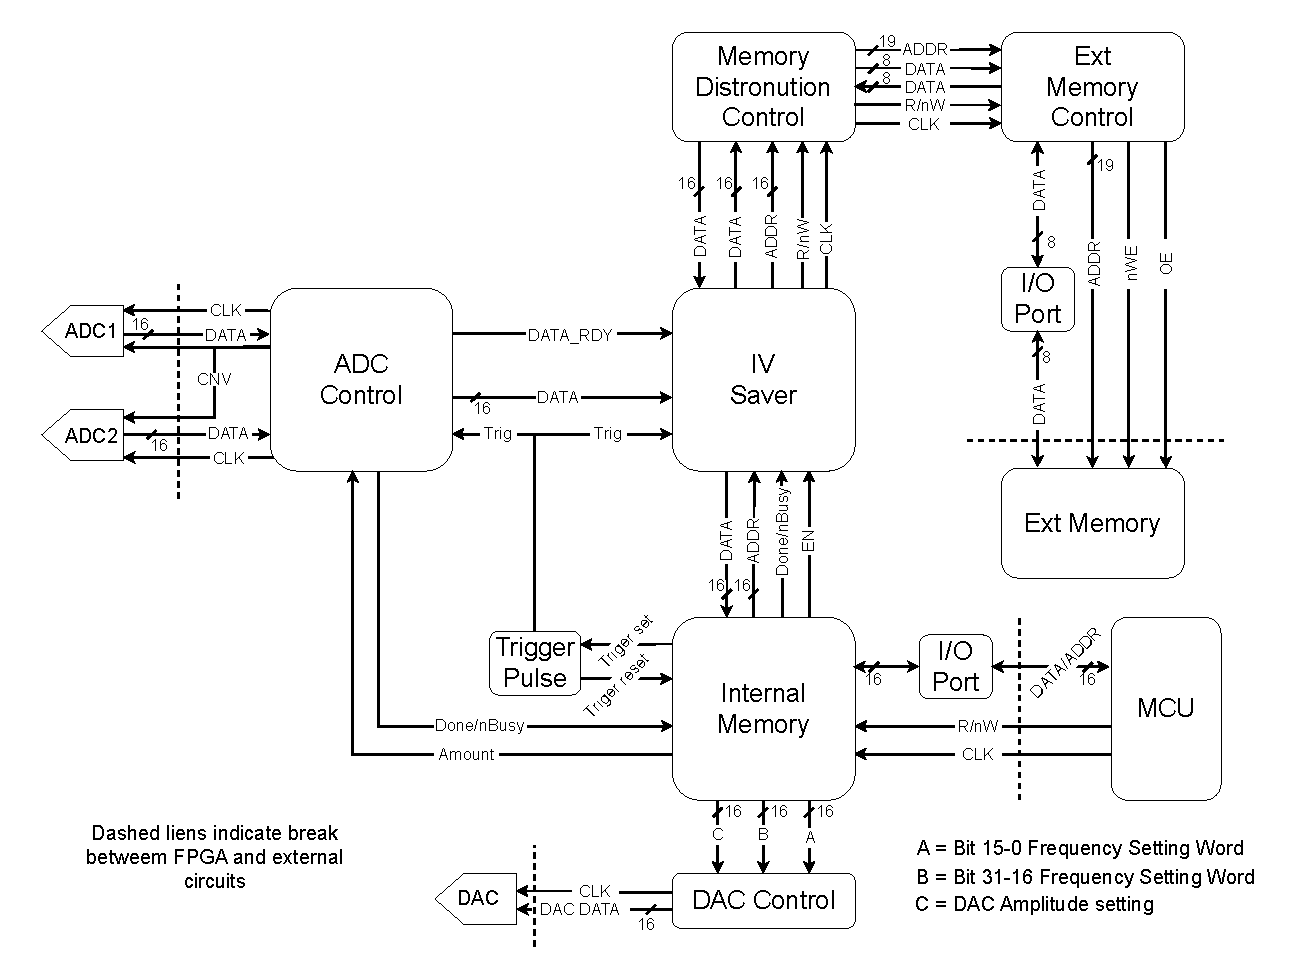
\includegraphics[clip, trim=0 0 0 0, width=1\textwidth]{Sections/7_SystemDesign/Figures/Sample_Control_Block.pdf}
    \caption{Block diagram of the internal logic blocks of the Sample Control Block.}
    \label{fig:7_SampleControlBlock}
\end{figure}

The block diagram on figure \refq{fig:7_SampleControlBlock} has a number of logic blocks. The MCU will connect to the Sample Control Module(SCM) through a parallel communication bus and it can do writes, or reads, to a number of internal registers in the Internal Memory block, and use these registers to adjust test parameters such as test frequency, sample rate, sample size and it can start a sampling process. 

The DAC Control block is controlling the stimulus inputs for the external DAC that is generating the test signal going into the DUT. The frequency of this DAC can be set in a register in the internal memory. A sampling process will start when the MCU has set a 'trigger' flag in a register in the internal memory. This register connects to the ADC Resampler logic and this logic will generate the acquisition signals for the ADC Control block. The ADC Resampler will generate an acquisition pulse for every sample until it has reached the desired sample size. The ADC Control logic will control the timing of the two ADCs necessary to sample the DUT voltage and current. It will sample the ADCs every time it recieves an acquisition input signal from the ADC Resampler and send the samples to the Parallel To Series Converter logic.

The two ADCs are sampled at the same time, but the external memory can store just one sample at a time. The Parallel To Series logic will take the two samples and trigger the IV Saver, Memory Distribution and External Memory Control logic twice, one for each sample, in order to cause these other logic blocks to save the two samples.

The IV Saver is a MUX that controls the input/output path to the external memory. During a sampling process it will forward data to the external memory through the Memory Distribution Control block, and when no sampling process is active, it will allow the MCU to read from the external memory.

The IX MUX block is a MUX that is connected to an input pin that the MCU can control. Depending on the state of this pin the MCU can access the internal memory registers, or it can read from the external memory through the IV Saver logic.

All the logic blocks on figure \refq{fig:7_SampleControlBlock} will be described in detail in this section.